\ExamPart{Trắc nghiệm nhiều phương án lựa chọn}{3.0}{Thí sinh trả lời từ câu 1 đến câu 12. Mỗi câu thí sinh chỉ chọn một phương án.}

\NQuestion Cho đồ thị hàm số $y=f\left(x\right)$ như hình vẽ dưới đây.
\begin{center}
    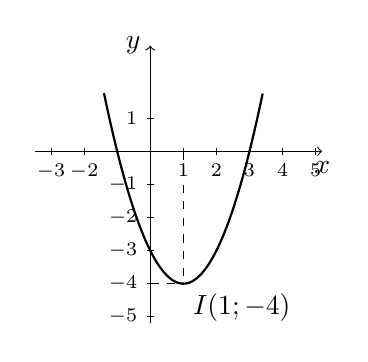
\begin{tikzpicture}[scale=0.42]
    \draw[->] (-3.5,0) -- (5.2,0) node[below] {$x$};
    \draw[->] (0,-5.2) -- (0,3.2) node[left] {$y$};

    \foreach \x in {-3,-2,1,2,3,4,5}
        \draw (\x,0.1) -- (\x,-0.1) node[below] {\scriptsize $\x$};

    \foreach \y in {-5,-4,-3,-2,-1,1}
        \draw (0.1,\y) -- (-0.1,\y) node[left] {\scriptsize $\y$};

    \draw[smooth, samples=200, domain=-1.4:3.4, thick]
        plot (\x, {\x*\x - 2*\x - 3});

    \draw[dashed] (1,0) -- (1,-4);
    \draw[dashed] (0,-4) -- (1,-4);
    \fill (-1,0) circle (1.3pt);
    \fill (3,0) circle (1.3pt);
    \fill (1,-4) circle (1.3pt);
    \node[below right] at (1,-4) {$I(1;-4)$};
\end{tikzpicture}

\end{center}
Tập nghiệm của bất phương trình $f\left(x\right)<0$ là
\ChoicesOneLine
{$(-\infty;-1)\cup(3;+\infty)$.}
{$(-1;3)$.}
{$[-1;3]$.}
{$(-\infty;-1]\cup[3;+\infty)$.}
{2}
\SolutionBlock{Từ đồ thị, parabol cắt trục hoành tại $x=-1$ và $x=3$, đồng thời mở lên. Vì vậy $f\left(x\right)<0$ khi $x$ nằm giữa hai nghiệm, tức là $x\in(-1;3)$.}

\NQuestion Tập nghiệm của bất phương trình $x^2-5x+6\ge 0$ là
\ChoicesOneLine
{$(-\infty;2)\cup(3;+\infty)$.}
{$[2;3]$.}
{$(-\infty;2]\cup[3;+\infty)$.}
{$(2;3)$.}
{3}
\SolutionBlock{Ta có $x^2-5x+6=(x-2)(x-3)$. Vì hệ số $a=1>0$ nên tam thức không âm ở ngoài khoảng giữa hai nghiệm và bằng $0$ tại $x=2,3$. Vậy tập nghiệm là $(-\infty;2]\cup[3;+\infty)$.}

\NQuestion Phương trình $\sqrt{x+2}=x$ có nghiệm là
\ChoicesOneLine
{$x=-1$.}
{$x=0$.}
{$x=2$.}
{$x=4$.}
{3}
\SolutionBlock{Điều kiện: $x\ge0$. Bình phương hai vế được $x+2=x^2\Leftrightarrow x^2-x-2=0\Leftrightarrow (x-2)(x+1)=0$. Đối chiếu điều kiện chỉ nhận $x=2$.}

\NQuestion Một nhà hàng có $4$ món khai vị, $3$ món chính và $2$ món tráng miệng. Số cách chọn một thực đơn gồm $1$ món khai vị, $1$ món chính và $1$ món tráng miệng là
\ChoicesOneLine{$9$.}{$12$.}{$18$.}{$24$.}{4}
\SolutionBlock{Áp dụng quy tắc nhân: có $4$ cách chọn món khai vị, $3$ cách chọn món chính và $2$ cách chọn món tráng miệng. Vậy có $4\cdot3\cdot2=24$ cách chọn.}

\NQuestion Số cách xếp $6$ học sinh phân biệt ngồi vào một hàng ghế là
\ChoicesOneLine{$120$.}{$360$.}{$720$.}{$840$.}{3}
\SolutionBlock{Số cách xếp $6$ học sinh phân biệt vào một hàng là số hoán vị của $6$ phần tử: $P_6=6!=720$.}

\NQuestion Từ các chữ số $0,1,2,3,4,5$, lập được bao nhiêu số tự nhiên chẵn có $4$ chữ số đôi một khác nhau?
\ChoicesOneLine{$120$.}{$156$.}{$180$.}{$216$.}{2}
\SolutionBlock{Xét chữ số hàng đơn vị.
\begin{itemize}[leftmargin=1.5em]
    \item Nếu hàng đơn vị là $0$ thì hàng nghìn có $5$ cách, hàng trăm có $4$ cách, hàng chục có $3$ cách. Có $5\cdot4\cdot3=60$ số.
    \item Nếu hàng đơn vị là $2$ hoặc $4$ thì có $2$ cách chọn. Khi đó hàng nghìn chọn từ $4$ chữ số khác $0$ và khác chữ số hàng đơn vị nên có $4$ cách; hàng trăm có $4$ cách; hàng chục có $3$ cách. Có $2\cdot4\cdot4\cdot3=96$ số.
\end{itemize}
Tổng cộng có $60+96=156$ số.}

\NQuestion Trong mặt phẳng tọa độ $Oxy$, cho $A(-1;2),\ B(3;5)$. Tọa độ vectơ $\overrightarrow{AB}$ là
\ChoicesOneLine{$(2;3)$.}{$(4;3)$.}{$(-4;-3)$.}{$(4;-3)$.}{2}
\SolutionBlock{Ta có $\overrightarrow{AB}=(3-(-1);5-2)=(4;3)$.}

\NQuestion Trong mặt phẳng tọa độ $Oxy$, trung điểm của đoạn thẳng nối hai điểm $M(2;-3)$ và $N(6;1)$ là
\ChoicesOneLine{$(4;-1)$.}{$(3;-1)$.}{$(8;-2)$.}{$(2;4)$.}{1}
\SolutionBlock{Trung điểm $I$ của đoạn $MN$ có tọa độ
\[
I\left(\dfrac{2+6}{2};\dfrac{-3+1}{2}\right)=(4;-1).
\]}

\NQuestion Trong mặt phẳng tọa độ $Oxy$, cho tam giác $ABC$ với $A(1;2),\ B(4;5),\ C(7;-1)$. Tọa độ trọng tâm $G$ của tam giác là
\ChoicesOneLine
{$\left(4;2\right)$.}
{$\left(\dfrac{4}{3};2\right)$.}
{$\left(4;\dfrac{2}{3}\right)$.}
{$\left(3;2\right)$.}
{1}
\SolutionBlock{Trọng tâm tam giác có tọa độ
\[
G\left(\dfrac{1+4+7}{3};\dfrac{2+5+(-1)}{3}\right)=(4;2).
\]}

\NQuestion Đường thẳng đi qua hai điểm $A(2;-1)$ và $B(4;3)$ có phương trình là
\ChoicesOneLine
{$2x-y-5=0$.}
{$2x+y-3=0$.}
{$x-2y+4=0$.}
{$x+2y=0$.}
{1}
\SolutionBlock{Ta có hệ số góc của $AB$ là $m=\dfrac{3-(-1)}{4-2}=2$. Phương trình đường thẳng qua $A(2;-1)$ là
\[
y+1=2(x-2)\Leftrightarrow 2x-y-5=0.
\]}

\NQuestion Cho đồ thị hàm số $y=f\left(x\right)$ như hình vẽ dưới đây.
\begin{center}
    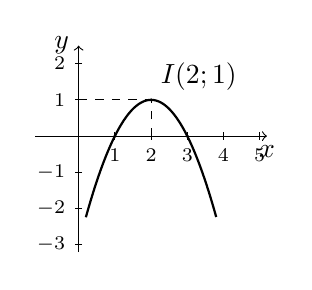
\begin{tikzpicture}[scale=0.46]
    \draw[->] (-1.2,0) -- (5.2,0) node[below] {$x$};
    \draw[->] (0,-3.2) -- (0,2.5) node[left] {$y$};

    \foreach \x in {1,2,3,4,5}
        \draw (\x,0.1) -- (\x,-0.1) node[below] {\scriptsize $\x$};

    \foreach \y in {-3,-2,-1,1,2}
        \draw (0.1,\y) -- (-0.1,\y) node[left] {\scriptsize $\y$};

    \draw[smooth, samples=200, domain=0.2:3.8, thick]
        plot (\x, {-\x*\x + 4*\x - 3});

    \fill (1,0) circle (1.3pt);
    \fill (3,0) circle (1.3pt);
    \fill (2,1) circle (1.3pt);
    \draw[dashed] (2,0) -- (2,1);
    \draw[dashed] (0,1) -- (2,1);
    \node[above right] at (2,1) {$I(2;1)$};
\end{tikzpicture}

\end{center}
Tập nghiệm của bất phương trình $f\left(x\right)\ge 0$ là
\ChoicesOneLine
{$[1;3]$.}
{$(-\infty;1]\cup[3;+\infty)$.}
{$(1;3)$.}
{$(-\infty;1)\cup(3;+\infty)$.}
{1}
\SolutionBlock{Từ đồ thị, parabol mở xuống và cắt trục hoành tại $x=1$ và $x=3$. Do đó $f\left(x\right)\ge0$ trên đoạn giữa hai nghiệm, tức là $[1;3]$.}

\NQuestion Gọi $\alpha$ là góc giữa hai đường thẳng $d_1:2x-y+1=0$ và $d_2:x+y-3=0$. Khi đó
\ChoicesOneLine
{$\tan\alpha=\dfrac13$.}
{$\tan\alpha=1$.}
{$\tan\alpha=2$.}
{$\tan\alpha=3$.}
{4}
\SolutionBlock{Ta có $d_1: y=2x+1$ nên $m_1=2$; $d_2: y=-x+3$ nên $m_2=-1$. Vậy
\[
\tan\alpha=\left|\dfrac{m_2-m_1}{1+m_1m_2}\right|=\left|\dfrac{-1-2}{1+2(-1)}\right|=3.
\]}
